\documentclass[../main.tex]{subfiles}
\begin{document}
\section{Corrections to simulated events}
\label{hh:sec:corrections}

In general, simulations do not perfectly reproduce the behaviour found in real data. To improve the agreement between data and simulated samples, somo correction factors or \textit{scale factors}  are included in the simulated events. These scale factors can modify the whole yield of particular samples (as the normalization factors obtained for Z$/\gamma^*\to ll$~+~jets or t$\bar{\text{t}}$ in Section~\ref{hh:sec:background}), weight each event independently according to some characteristics of the event, or even only modify particular objects in every event.

In the following, all the correction factors applied to simulated factors (except the normalization factors described in Section~\ref{hh:sec:background})) are summarised.

\subsubsection*{Pile-up reweighting}
\label{hh:sec:pu}

The production of additional objects coming from PU vertices can lead to variations in the analysis results. Therefore, the effect of additional proton-proton interactions is also modelled in simulated events. The probability distribution of the number of PU interactions is modelled before the data taking period itself. Therefore, simulated events have to be weighted according to the ratio between the PU distributions of data and MC. For the data, the pile-up is given by
\begin{equation}
\text{PU} = \frac{L_{ins}\cdot\sigma_{\text{inel}}}{\text{f}_\text{rev}},
\end{equation}
where $\sigma_{\text{inel}}$ is the total pp inelastic cross section and $\text{f}_\text{rev}$ is the LHC orbit frequency (11246~Hz). The cross section takes a value of 69.2~fb, as recommended by the Collaboration.

%\begin{figure}[h!]
%\begin{center}
%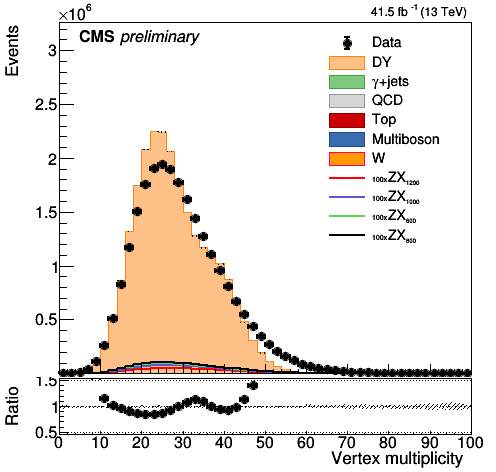
\includegraphics[width=0.5\textwidth]{Images/nvtx_mm.png}
%\end{center}
%\caption{Distribution of number of PU vertices in 2017 for both data and simulated samples.}
%\label{hh:fig:pu}
%\end{figure}

\subsubsection*{Pile-up jet identification scale factors}

As described in Section~\ref{hh:subsec:jets}, jets with $p_t < 50$~GeV only are considered if they satisfy the loose working point of the pile-up jet ID discriminator. As this discriminator is not 100\%(0\%) efficient on real(PU) jets and its results can differ between data and MC events, some scale factors are needed to weight each particular MC event. These scale factors are produced by studying the pile-up jet ID efficiency, i.e. probability of a real jet (a reconstructed jet matched to a MC generator-level jet) to pass the PU jet ID working point, and the mistag rate, i.e. the probability of a PU jet (a reconstructed jet not matched to a MC generator-level jet) to pass the PU jet ID working point.

\subsubsection*{Jet smearing}

Measurements have shown that the jet energy resolution (JER) in data is worse than in simulation \cite{hh:corr:smearing_8TeV}. Then, the four-momentum of the jets in simulated events need to be further smeared to describe the data. The smearing procedure consists on a hybrid method used to scale the reconstructed four-momentum of a jet with an scaling factor $f$. First, a matching is performed between the jet and a generator-level jet if $\Delta R(\text{jet}, \text{genjet})<0.2$ and $|p_T^{\text{jet}} - p_T^{\text{genjet}}| < 3\sigma p_T^{\text{jet}}$, where $\sigma$ is the relative jet momentum resolution measured in simulation. This resolution depends on the $p_t$ and $\eta$ of the jet and the measured PU. In case this matching is performed, the scaling factor $f$ is obtained as
\begin{equation}
f = 1 + (s - 1)\frac{p_T^\text{jet} - p_T^\text{genjet}}{p_T^\text{jet}},
\end{equation}
where $s$ is the data-to-simulation core resolution scale factor. Otherwise, $f$ is obtained in an stochastic approach as
\begin{equation}
f = 1 + N(0, \sigma)\sqrt{\max(s^2-1, 0)},
\end{equation}
where $N(0, \sigma)$ is a random number sampled from a normal distribution with zero mean and $\sigma$ standard deviation.

\subsubsection*{Level-1 ECAL prefiring}

In 2016 and 2017 operation, a slowly developing shift in the shape of the ECAL pulses was observed \cite{intro:l1_13tev}. This effect was manifested in an increasing offset in the timing calibration of the pulses related to the transparency loss of the ECAL crystals, mostly in the endcap. This offset was compensated offline by recalibrating the pulses, but was not corrected in the ECAL trigger primitives. With time, this effect ended up moving the endcap pulses to a time region where the bunch crossing assignment would be affected, leading to the Level-1 trigger system to \textit{prefire}, i.e. accept the earlier collision in BX - 1, whereas the one in BX 0 is the one of interest. Since Level-1 trigger rules forbid two consecutive bunch crossings to fire, the actual event would be skipped. This effect was not accounted for by the simulations, so additional weights are included to account for the probability of an event to prefire according to the $p_T$ and $\eta$ of forward jets and photons in the event. This weight is obtained as the product of the non prefiring probability of all jets and photons from the event:
\begin{equation}
w = \prod_{i\in \text{photons, jets}} (1 - \varepsilon_i^\text{pref}(p_T, \eta)).
\end{equation}

In early 2018, the endcap timing delays in the ECAL front-end electronics were corrected, optimizing the pulse synchronization and solving these prefiring issues.

\subsubsection*{Trigger efficiency scale factors}
\label{hh:sec:trigger_sf}

As the simulations do not reproduce exactly the data, there are some discrepancies obtained for the efficiencies obtained in the single-lepton, cross-lepton and VBF triggers used in the analysis. These discrepancies can be compensated by including some event weights.

For the \tauh\tauh{} final state, trigger efficiencies and scale factors are measured using Z~$\to$~\taumu\tauh{} events selected with a tag and probe technique, both in data and simulation. For the semi-leptonic final states, a similar technique is considered using Z$~\to\mu\mu$ and Z$~\to ee$ events. In these cases, the scale factors must take into account the logical OR of the single-lepton and cross-lepton triggers. Assuming the lepton and \tauh{} legs are independent, the efficiency for both simulation and data can be obtained as
\begin{equation}
\text{Eff} = \epsilon_L(1-\epsilon_{\tau_h}) +  \epsilon_l\epsilon_{\tau_h},
\end{equation}
where $\epsilon_L$ is the single lepton trigger efficiency, $\epsilon_l$ is the cross lepton trigger efficiency for the \taue{} or \taumu{} leg and $\epsilon_{\tau_h}$ is the cross lepton trigger efficiency for the \tauh{} leg.

For the VBF trigger paths, efficiencies and scale factors are computed separately for the \tauh{} legs and the jet legs. For the \tauh{} legs, a tag and probe technique focused on Z$~\to~$\taumu\tauh{} events is exploited. Both $\tau_h$ are considered independents, and their correspondent scale factors are obtained as a function of their $p_T$ and decay mode. For the jet legs, events are required to satisfy the requirements of one of the \tauh\tauh{} triggers considered and the additional requirements applied on the jets by the VBF trigger. The scale factors in this case are computed as a function of the transverse momenta of the two jets with the highest invariant mass and on the actual invariant mass. Note that these VBF trigger scale factors are only when at least one of the \tauh{} has a $p_T$ between 25 and 40~GeV. If both \tauh{} have a $p_t>40$~GeV, the $\tau_h\tau_h$ scale factors are considered instead.



\subsubsection*{Trigger prescale weights}
\label{hh:sec:prescale_sf}

In order to account for the prescales used for data taking for some of the HLT triggers, the simulated events that fired only prescaled paths are corrected with weights obtained as the ratio between the integrated luminosity covered by the prescaled trigger over the total integrated luminosity of the year.

Only two triggers used in the analysis were prescaled: the VBF triggers used in both 2017 and 2018. In the first case, out of the total 41.5~fb$^{-1}$ collected by the experiment, only 27.13~fb$^{-1}$ were taken with the trigger included. Then, simulated events that were selected as they satisfied this VBF trigger selection need to be weighted by around 0.65. Analogously, events that satisfied the 2018 VBF trigger selection are weighted by around 0.99.

\subsubsection*{b-tagging efficiency}

To account for discrepancies in the b-tagging performance of the DeepJet algorithm between data and simulation, the discriminant distribution is corrected by applying weights to the simulated events. These weights are obtained as
\begin{equation}
\label{hh:eq:btag_sf}
w = \prod_i^{N} SF(D^i, p_T^i, \eta^i),
\end{equation}
where $D^i$, $p_T^i$, and $\eta^i$ stand for the discriminator score, the transverse momentum and the pseudorapidity of the jet and the product  considers all jets satisfying the requirements described in Section~\ref{hh:subs:jets}. The scale factor for each jet are obtained as
\begin{equation}
SF(D^i, p_T^i, \eta^i) = \varepsilon^\text{data}(D^i, p_T^i, \eta^i)/\varepsilon^\text{MC}(D^i, p_T^i, \eta^i),
\end{equation}
where $\varepsilon^\text{data}(D^i, p_T^i, \eta^i)$ and $\varepsilon^\text{MC}(D^i, p_T^i, \eta^i)$ are the b-tagging efficiencies in data and simulation, respectively \cite{hh:analysis:btag}. In simulation, the b-tagging efficiency is defined as the number of identified b jets in a particular bin of the DeepJet discriminator, jet $p_T$ and jet $\eta$ with respect to the total number of b jets. The number of b jets is measured by matching the jets with the generated hadrons. In data, the tagging efficiency is measured using samples pure in b jets; e.g. a sample with high $p_T$ jets with a muon inside them (a topology usually found in heavy-flavour jets), or a di-lepton plus jets sample, expected to include b jets coming from top quark decays. To account for possible misidentification of jets in real data, the misidentification probability obtained from simulation is subtracted from the tagging efficiency in data. This misidentification probability is obtained as the number of jets misidentified as b jets and matched to generated non-b jets out of the total jets matched to generated non-b jets.

As stated before, these additional weights intend to only modify the shape of distribution, not the expected event yields. As only applying these weights could lead to modification on the total event yields, the final distributions are corrected by scaling with the ratio of the sum of event weights without considering the b-tag weight and considering it.

\subsubsection*{\deeptau{} scale factors}

The \deeptau{} algorithm shows small differences when running it on data or simulated events. To account for these differences, some scale factors are included depending on if a genuine $\tau_h$ or a misidentified particle is selected as the $\tau_h$ \cite{tau_performance_2022}. 

For genuine $\tau_h$, scale factors are computed with a tag and probe technique by selecting Z~$\to\tau\tau$ events decaying into a \taumu\tauh{} final state. Several quality cuts are applied to both $\mu$ and $\tau_h$ to increase the signal purity. Two sets of scale factors are then computed, either binned in the \tauh{} $p_t$ or in its decay mode. In the bb$\tau\tau$ analysis, the former is used for all \tauh{}, modifying the event weight.

For genuine electrons and muons misidentified as $\tau_h$, scale factors are computed with a tag and probe technique by selecting Z~$\to$ee and Z~$\to\mu\mu$ events, respectively, where one of the leptons is correctly reconstructed and the other is reconstructed as a $\tau_h$. For electrons, scale factors are provided split into barrel and endcap, while for muons, binned as a function of $\eta$.

\subsubsection*{Electron and muon scale factors}

To account for possible disagreements between data and simulation regarding the reconstruction and identification of muons and electrons in the \taumu\tauh{} and \taue\tauh{} channels, specific scale factors binned in the lepton $p_t$ and $\eta$ are provided. Scale factors are obtained with tag and probe techniques, selecting Z~$\to$~ee and Z~$\to\mu\mu$ events.

\subsubsection*{Tau Energy Scale}

The correction to the $\tau_h$ energy scale is defined by the deviation of the average reconstructed $\tau_h$ energy from the generator-level energy of the visible \tauh{} decay products \cite{tau_performance_2018, tau_performance_2022}. The data-to-simulation correction factor is obtained by fitting distributions of observables sensitive to the $\tau_h$ energy scale in Z/$\gamma^*\to\tau\tau\to\tau_e\tau_h,~\tau_\mu\tau_h$, such as the $m_{\tau_h}$ and the mass of the $l\tau_h$ system. These corrections modify the energy and momentum on the $\tau_h$, modifying also the shape of the final discriminants. Four independent corrections are provided, one for each decay mode used in the analysis, taking values of up to 2\%. 


\end{document}

